% Compile: pdflatex main && bibtex main && pdflatex main && pdflatex main
\documentclass{article}

% Official NeurIPS 2026 workshop style (anonymous / double-blind).
\usepackage[dblblindworkshop]{neurips_2026}
\workshoptitle{Machine Learning and the Physical Sciences}

\usepackage[utf8]{inputenc}
\usepackage[T1]{fontenc}
\usepackage{amsmath,amssymb,amsfonts}
\usepackage{booktabs}
\usepackage{graphicx}
\usepackage{hyperref}
\usepackage{url}
\usepackage{microtype}
\usepackage{xcolor}

\title{Shared Structure Through Alignment:\\
Testing Platonic Scaling in Cross-Survey Astronomy}

\author{Anonymous Author(s)}

\begin{document}

\maketitle

\begin{abstract}
The Platonic Representation Hypothesis predicts increasing representational convergence with model scale, but the observed trend depends on how cross-system correspondence is measured.
We study matched Legacy Survey and HSC astronomical embeddings across five model families and sixteen model-size rungs.
A supervised dense linear alignment substantially increases held-out neighbourhood correspondence and steepens its dependence on model size relative to native cosine geometry: the slope increase is positive in all five families (\(T{=}0.00721\)), survives an object-level bootstrap (95\% CI \([0.0034,0.0111]\)), and exceeds a synchronized correspondence-shuffle refit null (\(p{=}1/201\approx0.005\)).
The effect is not explained by rotation or change of basis; the learned maps remain strongly anisotropic with size, with most useful transfer concentrated in a small leading singular subspace.
PCA bottlenecks further improve alignment level but do not clearly strengthen scaling, while sparse SAE and BSF representations do not outperform the matched dense-alignment baseline.
These results suggest that model scaling increases linearly recoverable cross-survey structure without driving the representations toward a common isometric geometry.
\end{abstract}

\section{Introduction}
\label{sec:intro}

Representations from independently trained models often become more aligned as capability and scale increase~\citep{huh2024platonic}.
The Platonic Representation Hypothesis (PRH) interprets this as convergence toward a shared statistical model of reality.
In astronomy, matched survey embeddings give a comparatively clean test: prior work reports increasing mutual \(k\)-nearest-neighbour (mKNN) agreement with model capacity on Legacy Survey~\citep{dey2019legacy}\(\leftrightarrow\)HSC~\citep{miyazaki2018hsc} ladders~\citep{duraphe2025platonicuniverse}.

A strong reading of Platonic convergence asks whether Legacy and HSC embeddings \(X_L\) and \(X_H\) become directly geometrically similar.
A weaker, but often more operational, reading asks whether they become increasingly equivalent under a restricted transformation class \(T(X_L)\approx X_H\).
We organize allowed maps as
\(\mathcal T_{\mathrm{id}}\subset\mathcal T_{\mathrm{similarity}}\subset\mathcal T_{\mathrm{linear}}\):
identity/native geometry; rotation/reflection plus uniform scaling (similarity/isometric class), which preserves all pairwise cosines and therefore cosine \(k\)NN structure; and general linear maps, which can apply direction-dependent stretch.
PCA is treated as a \emph{bottleneck before} linear alignment rather than as another nested geometric class.
We distinguish three measurements on the same held-out objects:
\emph{native correspondence} \(M_{\mathrm{Dense}}\) (cosine geometry in the original coordinates);
\emph{linearly recoverable correspondence} \(M_{\mathrm{Dense+Ridge}}\) (after a supervised global linear map fit on paired training objects);
and \emph{bottleneck-assisted recoverability} \(M_{\mathrm{PCA+Ridge}}\) (independent survey PCAs before the same map).
We also evaluate sparse SAE~\citep{gao2025sae}/BSF~\citep{fel2026bsf} representations with matched Ridge supervision and---as a complementary construction---an unpaired nonlinear shared bottleneck~\citep{jha2025vec2vec}.

The central empirical question is which notion of cross-survey equivalence exhibits model-size scaling.
We find that supervised linear recoverability shows substantially stronger size dependence than native cosine geometry, without evidence that the required maps approach rotations or other similarity transforms.

\section{Setup}
\label{sec:setup}

We use the official UniverseTBD Legacy\(\leftrightarrow\)HSC matched embeddings~\citep{duraphe2025platonicuniverse} (\(n{=}16{,}384\) objects) across five families---AstroPTv2~\citep{smith2024astropt}, ConvNeXtv2~\citep{woo2023convnextv2}, DINOv2~\citep{oquab2024dinov2}, ViT~\citep{dosovitskiy2021vit}, and I-JEPA~\citep{assran2023ijepa}---sixteen size rungs in total (Appendix~\ref{app:details}).
I-JEPA has only two rungs; its slopes are two-point.

For representations \(A\) and \(B\),
\[
M_k=\frac{1}{n}\sum_i
\frac{\lvert \mathcal N_k^A(i)\cap \mathcal N_k^B(i)\rvert}{k},
\]
with cosine neighbours and self-exclusion~\citep{huh2024platonic,duraphe2025platonicuniverse}.
The primary scale is \(k{=}10\).
All primary results use a frozen train/test split (\(n_{\mathrm{train}}{=}13{,}107\), \(n_{\mathrm{test}}{=}3277\), seed \(0\)) and a \textbf{test-only gallery}: neighbours are sought among held-out objects only (chance \(\approx 10/3276\approx0.0031\)).
Direction is Legacy\(\to\)HSC.

Dense Ridge fits \(\mathrm{StandardScaler}\) on train \(X,Y\) then Ridge with \(\alpha{=}1\) and an intercept, matching the supervision used for SAE/BSF maps.
PCA+Ridge fits independent survey PCAs on an inner training subset (as in our controls), then the same Ridge recipe.
Raw-PCA controls instead use a single pooled PCA basis on stacked train embeddings from both surveys---without object pairing---and raw cosine afterwards (Appendix~\ref{app:pca}).

\section{Alignment exposes stronger scaling}
\label{sec:scaling}

Mean held-out mKNN@10 is \(0.022\) for raw Dense, \(0.042\) for Dense+Ridge, \(0.033\) for SAE+Ridge, and \(0.035\) for BSF+Ridge (Figure~\ref{fig:scaling}).
Dense+Ridge therefore raises recoverable correspondence relative to native geometry.
It also steepens family OLS slopes of mKNN versus \(\log_{10}P\):
\[
\Delta\beta_F=\beta_{\mathrm{Dense+Ridge},F}-\beta_{\mathrm{Dense},F}
\]
is positive in all five families
(AstroPT \(+0.0051\), ConvNeXt \(+0.0029\), DINOv2 \(+0.0031\), ViT \(+0.0103\), I-JEPA \(+0.0146\)).
The primary aggregate is
\[
T=\frac15\sum_F\Delta\beta_F=0.00721.
\]
Adjacent within-family interactions \(D=\Delta M_{\mathrm{Dense+Ridge}}-\Delta M_{\mathrm{Dense}}\) are positive on \(9/11\) transitions (mean \(+0.0026\)).

Three complementary tests support this amplification (Appendix~\ref{app:stats}).
A one-sided exact sign test on the five family signs gives \(p=(1/2)^5=0.03125\).
A synchronized shuffle-refit null (\(B{=}200\)) permutes training Legacy\(\leftrightarrow\)HSC correspondences once per draw, refits Ridge on every rung, and recomputes \(T\): the null mean is \(-0.017\), none of \(200\) draws meet or exceed \(T_{\mathrm{real}}\), so \(p_{\mathrm{perm}}=1/201\approx0.005\).
An object bootstrap (\(B{=}5000\)) resampling the same held-out IDs across all rungs/methods yields a \(95\%\) CI \([0.0034,0.0111]\) for \(T\); excluding I-JEPA (\(T_{-I}=\) mean over four families) gives \(T_{-I}=0.00537\) with all four remaining families positive.
These ask different questions---architecture-level direction, necessity of true pairing for the scaling statistic, and object-level robustness---and are not interchangeable nulls.

\paragraph{Fixed-rank control.}
To separate representation dimension from alignment capacity, we repeat the comparison at matched PCA rank \(r{=}256\) with independent survey PCAs (Appendix~\ref{app:fixedrank}).
Raw PCA256 native mKNN and PCA256+Ridge use the same 256-dimensional representations; defining
\(\Delta\beta_{F,256}=\beta_{\mathrm{PCA256+Ridge},F}-\beta_{\mathrm{PCA256},F}\),
we obtain \(T_{256}=0.00864\) with \(\Delta\beta_{F,256}>0\) in all five families (sign test \(p{=}0.03125\); \(T_{256}^{(-I)}=0.00673\)).
Supervised recoverability therefore steepens with model size even at equal bottleneck dimension.

Supervised linear alignment therefore amplifies the model-size dependence of recoverable cross-survey correspondence.
This is not unsupervised convergence: object pairing is used to fit the map.

\begin{figure}[t]
\centering
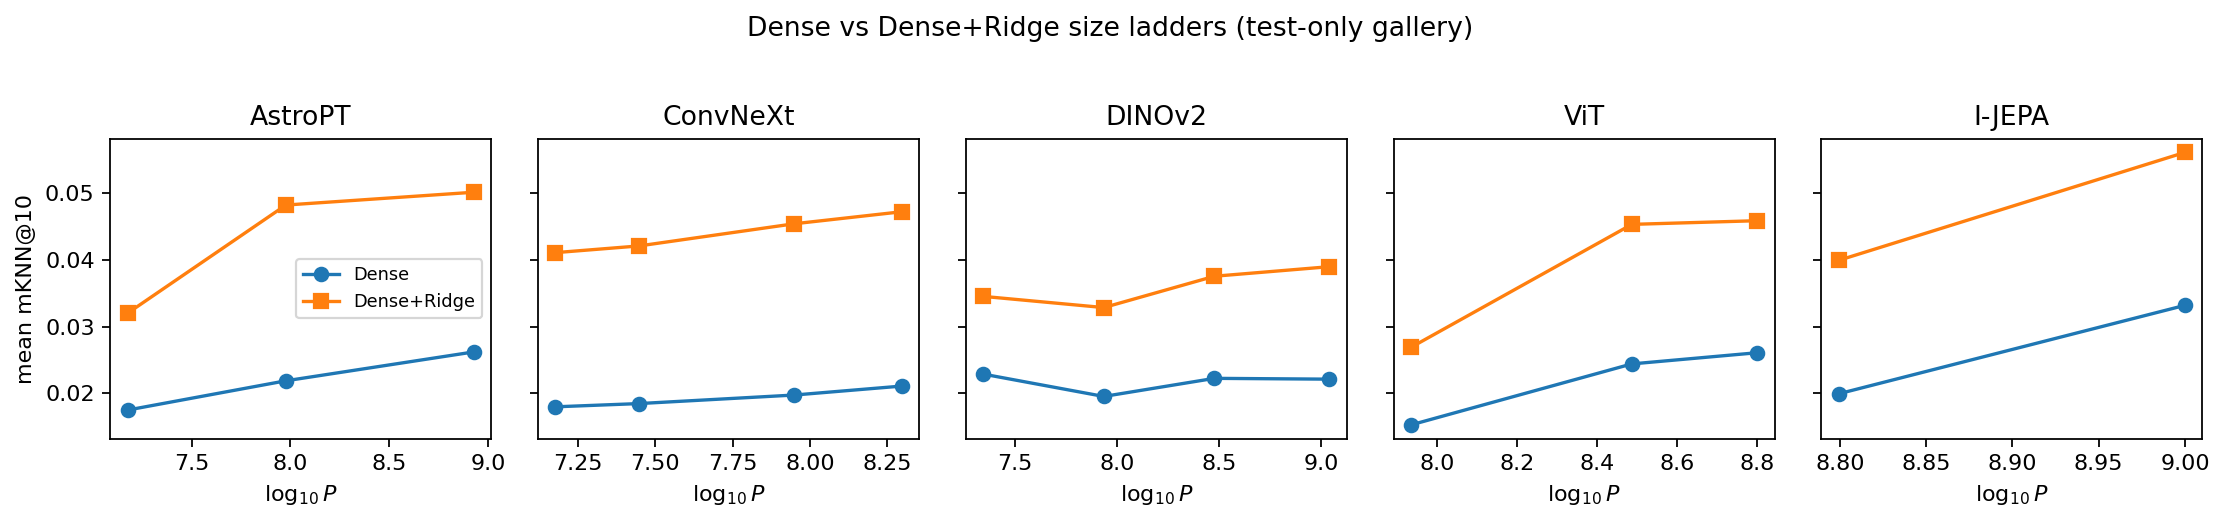
\includegraphics[width=\linewidth]{figures/dense_vs_ridge_scaling.png}
\caption{Held-out mKNN@10 versus \(\log_{10}P\) (test-only gallery).
Dense+Ridge raises the level and steepens the size trend relative to raw Dense in all five architecture families.}
\label{fig:scaling}
\end{figure}

\section{What kind of alignment?}
\label{sec:geometry}

\paragraph{Beyond similarity transforms.}
Because cosine neighbourhoods are invariant to a global orthogonal transformation, any increase in mKNN necessarily requires a map that changes native metric geometry.
We therefore characterize the learned linear alignment by its effective end-to-end singular spectrum and by empirical local stretch on held-out Legacy edges (Appendix~\ref{app:geometry}).

\paragraph{Strong anisotropic deformation.}
Ridge is fit after train-only \(\mathrm{StandardScaler}\) on \(X,Y\); we analyze the composed end-to-end map
\(A=\mathrm{diag}(\sigma_y)W\mathrm{diag}(1/\sigma_x)\) in original coordinates
(\(W{=}\)Ridge \(\texttt{coef\_}\)), not \(W\) alone in standardized space.
Writing \(y\approx Ax+b\) and taking the SVD of \(A\), geometric-mean--normalized singular spectra remain far from flat:
\(A_{\log}=\mathrm{std}(\log\tilde\sigma)\approx1.76\)--\(3.15\) (typically \(\approx1.76\)--\(1.93\)),
distance from a similarity transform \(D_{\mathrm{sim}}\approx0.89\)--\(1.00\),
and normalized spectral entropy \(H_{\mathrm{norm}}\) typically \(\approx0.21\)--\(0.58\) with a few feature-scale--dominated near-degeneracies (\(H_{\mathrm{norm}}{=}1\) is perfectly flat energy).
Family slopes of \(H_{\mathrm{norm}}\) versus \(\log_{10}P\) are mixed (\(2\) increasing, \(3\) decreasing), and recoverability versus \(H_{\mathrm{norm}}\) has Spearman \(\rho\approx0.04\) across rungs.
Alignment becomes more successful with model size without becoming more isotropic (Figure~\ref{fig:geometry}b).

\paragraph{Data-supported distortion.}
On held-out Legacy test edges (\(k_{\mathrm{edge}}{=}10\)), local log-stretch
\(s_{ij}=\log(|A_{\mathrm{eff}}\delta_{ij}|/|\delta_{ij}|)\)
has per-rung standard deviation \(\sigma_{\mathrm{local}}\approx0.16\)--\(0.31\) (Appendix~\ref{app:geometry}).
A scaled isometry would give constant \(s_{ij}\); the observed spread confirms direction-dependent deformation on the empirical manifold, not only in unused ambient directions.
Family slopes of \(\sigma_{\mathrm{local}}\) versus \(\log_{10}P\) are mixed, so increased recoverability is not accompanied by consistent local metric simplification.

\paragraph{Functionally concentrated maps.}
Truncating the fitted map \(A\) (no refit) shows that roughly \(6\%\) of singular directions recover at least \(90\%\) of the Dense+Ridge mKNN lift.
This concerns the learned map, not the intrinsic rank of the embeddings: most functional contribution to neighbourhood transfer lies in a small leading singular subspace despite global anisotropy.

\paragraph{PCA assists recoverability, not native similarity.}
Independent-PCA+Ridge improves the \emph{level} of recoverable correspondence at mid/high ranks (mean mKNN \(\approx0.044/0.050/0.055\) at ranks \(128/256/512\); \(512\) on \(14/16\) rungs with sufficient dimension), rising through the tested ladder rather than peaking at an ultra-low rank (Appendix~\ref{app:pca}).
A pooled shared-basis raw-PCA control---fit without pairing---barely changes native mKNN (\(\approx0.024\) at rank \(256\) versus \(0.022\) for Dense), so PCA does not substantially make the surveys more similar in projected native geometry.
The PCA\(\times\)Ridge interaction
\(I=(M_{\mathrm{PCA+Ridge}}-M_{\mathrm{rawPCA}})-(M_{\mathrm{Dense+Ridge}}-M_{\mathrm{Dense}})\)
is positive at ranks \(256\) and \(512\) (\(\approx{+}0.006\) and \(\approx{+}0.010\)), indicating that dimensional reduction specifically increases structure recoverable by the supervised map.
Relative to Dense+Ridge, PCA does not clearly add a robust further scaling interaction (only \(3/5\) families positive at \(256/512\)).
The central scaling phenomenon remains Dense+Ridge versus raw Dense.

\paragraph{Sparse representations as negative controls.}
Earlier SAE/BSF lifts over raw Dense confounded representation change with supervised alignment.
With supervision matched,
\(S_R=M_{R+\mathrm{Ridge}}-M_{\mathrm{Dense+Ridge}}\)
averages \(-0.0085\) for SAE (95\% family-bootstrap CI \([-0.0120,-0.0043]\); \(1/16\) positive) and \(-0.0062\) for BSF (95\% CI \([-0.0104,-0.0007]\); \(4/16\) positive).
Dense+Ridge beats SAE on \(15/16\) rungs and BSF on \(12/16\).
Against Dense+Ridge, SAE slope differences are negative in \(4/5\) families and adjacent controlled interactions are mixed (\(4/11\) SAE, \(6/11\) BSF positive).
Sparse SAE/BSF representations do not expose additional cross-survey correspondence beyond an equally supervised dense alignment, and we find no consistent positive sparse-representation\(\times\)scale interaction beyond that baseline (Figure~\ref{fig:geometry}c).

\paragraph{Unpaired nonlinear bottleneck.}
As a complementary construction that does not use paired cross-survey training objects, a DualEncoder shared latent bottleneck~\citep{jha2025vec2vec} recovers above-chance relational correspondence with non-monotonic size dependence (Appendix~\ref{app:unpaired}).
Recoverability therefore depends strongly on the allowed alignment class; the clean size law in these experiments is specific to paired linear recoverability.

\begin{figure}[t]
\centering
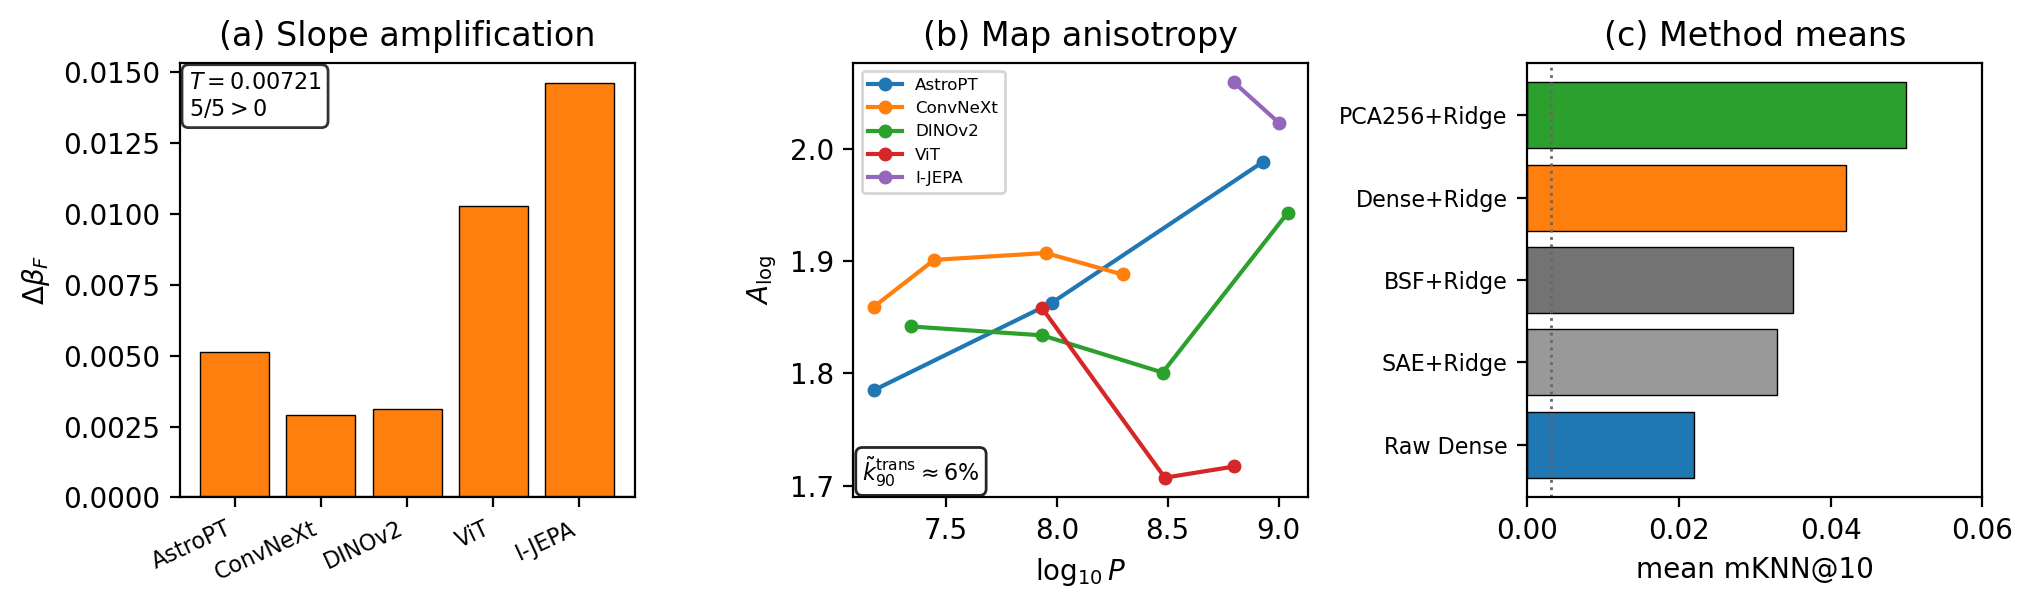
\includegraphics[width=\linewidth]{figures/alignment_geometry_summary.png}
\caption{(a)~Family slope amplifications \(\Delta\beta_F\) (all positive; \(T{=}0.00721\)).
(b)~Singular-spectrum anisotropy \(A_{\log}\) versus model size (maps remain strongly anisotropic).
(c)~Mean held-out mKNN@10 by method (test-only gallery; dotted: chance).}
\label{fig:geometry}
\end{figure}

\section{Discussion and conclusion}
\label{sec:disc}

The distinction is between native geometric similarity and recoverability under a transformation class.
Raw cosine asks whether the two survey representations already induce similar neighbourhood geometry.
Ridge asks how much correspondence is accessible after a supervised global linear deformation.
The latter exhibits substantially stronger model-size dependence, yet the required maps remain highly anisotropic and do not approach orthogonal or similarity transforms.
Scaling therefore increases recoverable common structure without producing evidence that the representations converge toward a shared metric geometry.
PCA further increases recoverability despite little effect on native correspondence, suggesting---as a hypothesis rather than a mechanism---that some dense directions interfere with alignment rather than contribute to shared geometry.

Limitations include paired supervision for the main Ridge result, five architecture families (I-JEPA two-rung), a single astronomy cross-survey setting, fixed Ridge \(\alpha{=}1\) (robustness to other \(\alpha\) in Appendix~\ref{app:fixedrank}), and incomplete exploration of local/nonlinear maps and PCA mechanisms.
Weak residual locality after global Ridge is measurable but small and is deferred to Appendix~\ref{app:stats}.

In summary: (i)~paired linear recoverability scales with model size more clearly than native cosine geometry;
(ii)~the required transformation remains strongly anisotropic;
(iii)~compression and sparse representation choices change the level of recoverability but do not overturn the central Dense+Ridge versus Dense scaling law.
These results support a weaker notion of Platonic convergence: larger models encode increasingly recoverable shared structure across surveys, even when their native representational geometries remain substantially different.

{\small
\bibliographystyle{plainnat}
\bibliography{references}
}

\appendix
\section{Protocol details and statistics}
\label{app:details}
\label{app:stats}

\paragraph{Ladders.}
Approximate parameter counts (\(10^{6}\)):
AstroPTv2 \(15/95/850\);
ConvNeXtv2 nano/tiny/base/large \(15/28/89/198\);
DINOv2 small/base/large/giant \(22/86/300/1100\);
ViT base/large/huge \(86/307/632\);
I-JEPA huge/giant \(630/1000\).

\paragraph{SAE/BSF.}
SAE width \(F{=}2048\), seed \(0\), TopK from available checkpoints (\(k\in\{18,\ldots,23\}\)), train-only Ridge and IDF, fixed Legacy\(\to\)HSC side.
BSF uses Vanilla signed codes with the same shared-basis Ridge protocol.

\paragraph{Complementary tests for \(T\).}
Family sign test: architecture-level directional consistency (\(n{=}5\)).
Synchronized shuffle-refit: one permutation seed defines a coherent shuffled training correspondence applied across all sixteen rungs; Dense slopes stay fixed while shuffled-Ridge slopes enter \(T_b\).
Object bootstrap: resample test IDs with replacement, recompute mean mKNN per rung/method, refit family slopes, and recompute \(T\).

\paragraph{Residual locality.}
Global Ridge residuals on test objects are locally structured in source space (\(k\in\{10,25,50\}\)): all \(16{\times}3\) residual-permutation tests give \(p{=}1/201\), but absolute residual cosine similarity is \(\approx0.01\) and trends versus size are mostly flat.
A weak location-dependent correction remains; we do not fit local maps here.

\section{PCA and raw-PCA controls}
\label{app:pca}

\begin{figure}[t]
\centering
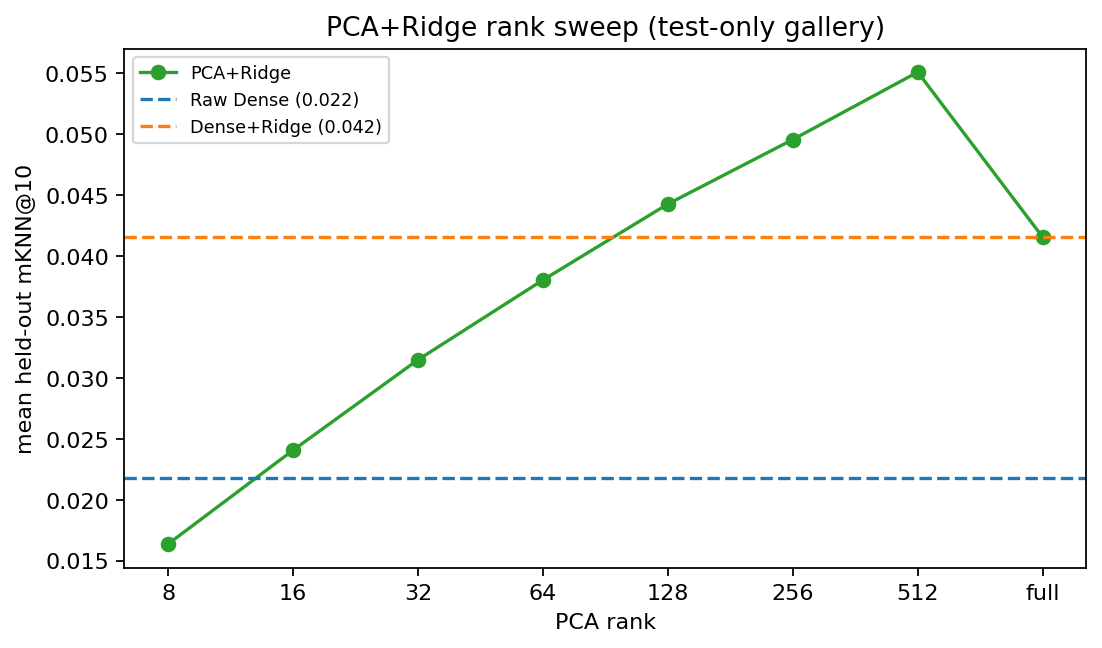
\includegraphics[width=0.85\linewidth]{figures/final_pca_mean_mknn_vs_rank.png}
\caption{Independent-PCA+Ridge mean mKNN versus rank (test-only gallery), with horizontal references for raw Dense and Dense+Ridge.
Performance rises through mid/high ranks; full Dense+Ridge underperforms PCA\(128\)--\(512\).}
\label{fig:pca-rank}
\end{figure}

\begin{figure}[t]
\centering
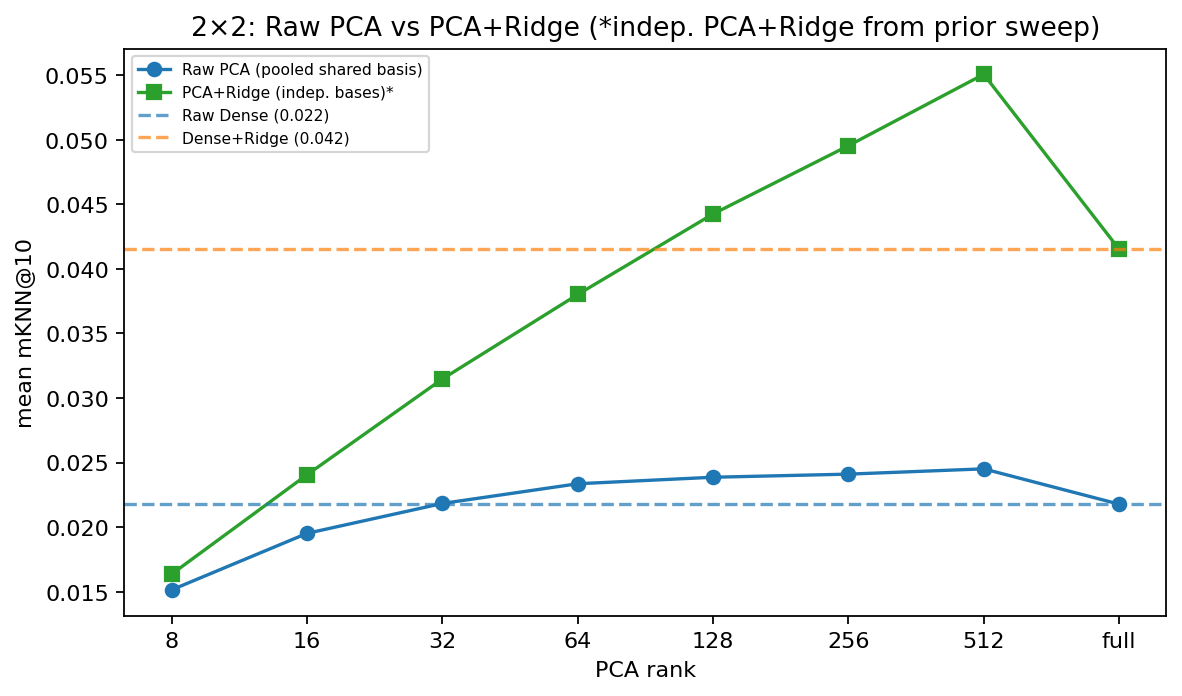
\includegraphics[width=0.85\linewidth]{figures/raw_pca_rank_curve.png}
\caption{Pooled shared-basis raw PCA versus independent-PCA+Ridge.
Raw PCA stays near Dense; almost all of the PCA headline requires Ridge.}
\label{fig:raw-pca}
\end{figure}

Independent-PCA+Ridge means (test-only): ranks \(8\)--\(64\) mostly below Dense+Ridge; rank \(128\) \(\approx0.044\) (\(13/16\) above Dense+Ridge); rank \(256\) \(\approx0.050\) (\(16/16\)); rank \(512\) \(\approx0.055\) (\(14/14\) valid).
Pooled raw PCA at rank \(256\): mean \(\approx0.024\) versus Dense \(0.022\).
PCA\(\times\)Ridge interaction means: \(\approx{+}0.006\) at \(256\) (\(14/16\) positive) and \(\approx{+}0.010\) at \(512\) (\(14/14\)).
Raw PCA does not steepen native family slopes relative to Dense.

\section{Fixed-rank scaling and Ridge-\texorpdfstring{$\alpha$}{alpha} robustness}
\label{app:fixedrank}

\begin{figure}[t]
\centering
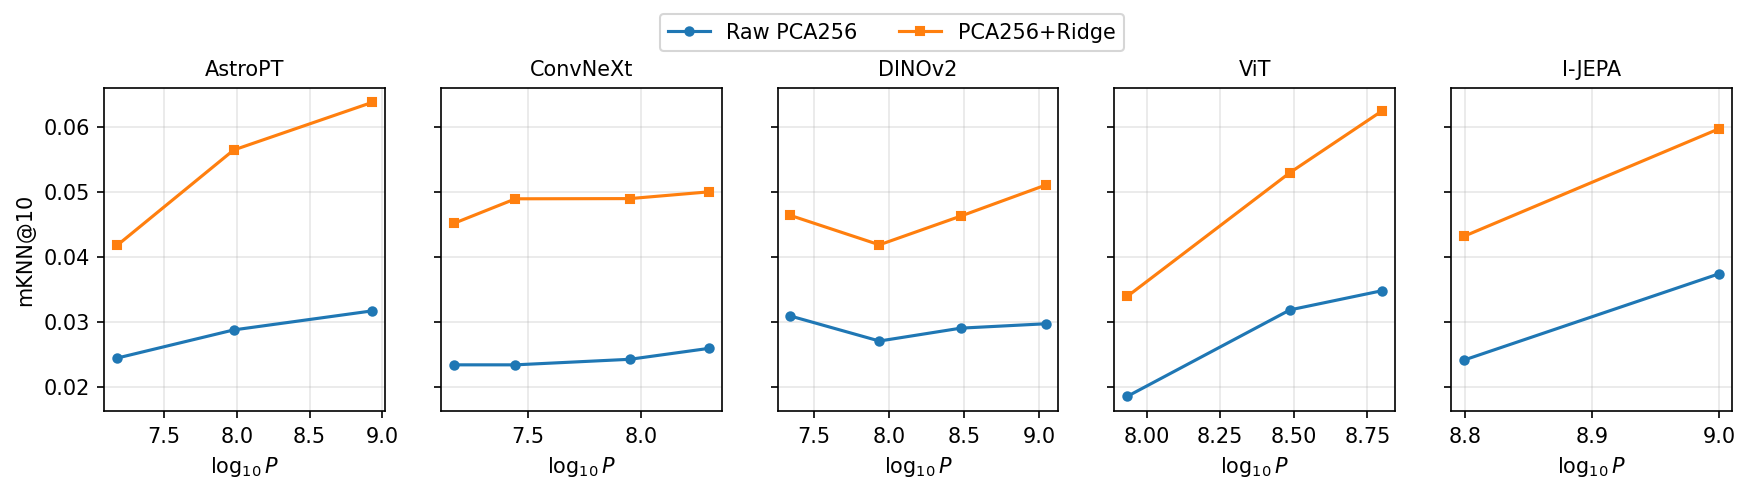
\includegraphics[width=\linewidth]{figures/fixed_rank_256_scaling.png}
\caption{Fixed rank \(256\): raw independent-PCA mKNN versus PCA256+Ridge by family (test-only gallery).
Ridge steepens the size dependence at matched representation dimension.}
\label{fig:fixedrank}
\end{figure}

At PCA rank \(256\) with independent survey bases, \(T_{256}=0.00864\) and all five families have \(\Delta\beta_{F,256}=\beta_{\mathrm{PCA256+Ridge},F}-\beta_{\mathrm{PCA256},F}>0\) (sign test \(p{=}0.03125\)).
Excluding I-JEPA, \(T_{256}^{(-I)}=0.00673\) with four/four positive.
At rank \(128\), \(T_{128}=0.00227\) with three/five positive (weaker, as expected at a tighter bottleneck).

Ridge regularization sweep (\(\alpha\in\{0.01,0.1,1,10,100\}\), no tuning on test):
\(T(\alpha)\in[0.0072,0.0085]\) with all five families positive at every tested \(\alpha\).

\section{Map geometry definitions and local distortion}
\label{app:geometry}

\paragraph{Effective map and spectral metrics.}
After train-only \(\mathrm{StandardScaler}\), Ridge yields \(W\); the analyzed end-to-end map is
\(A_{\mathrm{eff}}=\mathrm{diag}(\sigma_y)W\mathrm{diag}(1/\sigma_x)\).
Let \(\tilde\sigma_i\) be singular values normalized by their geometric mean.
We report
\(A_{\log}=\mathrm{std}(\log\tilde\sigma_i)\),
\(D_{\mathrm{sim}}=\min_{c,Q^\top Q=I}|A-cQ|_F/|A|_F\) (optimal \(Q^\star=UV^\top\) for \(A=U\Sigma V^\top\)),
and normalized spectral entropy \(H_{\mathrm{norm}}=-\sum_i p_i\log p_i/\log d\) with \(p_i=\sigma_i^2/\sum_j\sigma_j^2\).

\paragraph{Local stretch on held-out edges.}
Within the Legacy test gallery, each point's \(k_{\mathrm{edge}}\)-NN edges give \(\delta_{ij}=x_j-x_i\) and
\(s_{ij}=\log(|A_{\mathrm{eff}}\delta_{ij}|/|\delta_{ij}|)\).
We summarize \(\sigma_{\mathrm{local}}=\mathrm{std}(s_{ij})\) and robust spread \(R_{\mathrm{local}}=Q_{0.90}-Q_{0.10}\).

\begin{figure}[t]
\centering
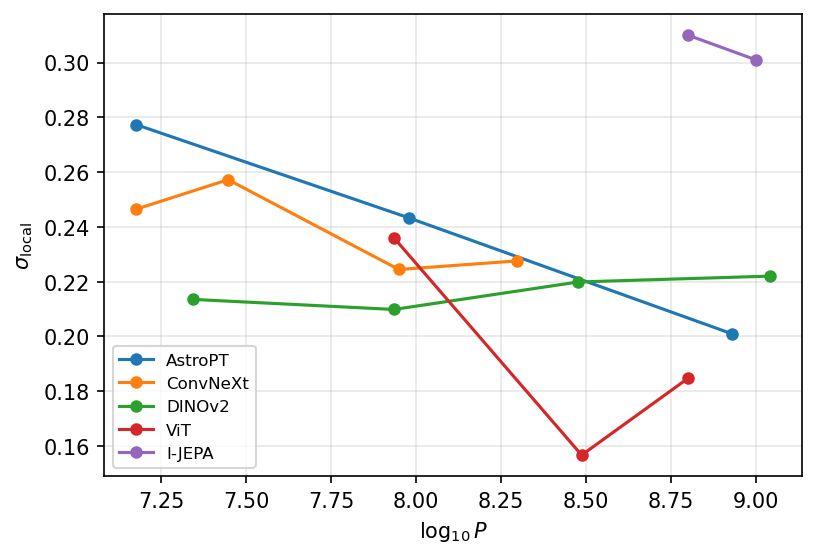
\includegraphics[width=0.72\linewidth]{figures/local_edge_distortion_vs_size.png}
\caption{Data-supported local distortion \(\sigma_{\mathrm{local}}\) versus \(\log_{10}P\) (\(k_{\mathrm{edge}}{=}10\)).}
\label{fig:localdist}
\end{figure}

\section{Unpaired relational alignment}
\label{app:unpaired}

Each survey is mapped through a model-specific MLP into a shared latent \(Z{=}256\) and decoded back, trained without paired cross-survey objects (reconstruction, RBF-MMD, cycle, and Gram terms; Appendix protocol as previously reported).
Held-out relational mKNN@10 lies in \(0.012\)--\(0.023\) versus chance \(\approx0.0035\), with non-monotonic size dependence on available ConvNeXt and DINOv2 ladders (\(2/6\) adjacent steps positive; Figure~\ref{fig:unpaired}).

\begin{figure}[t]
\centering
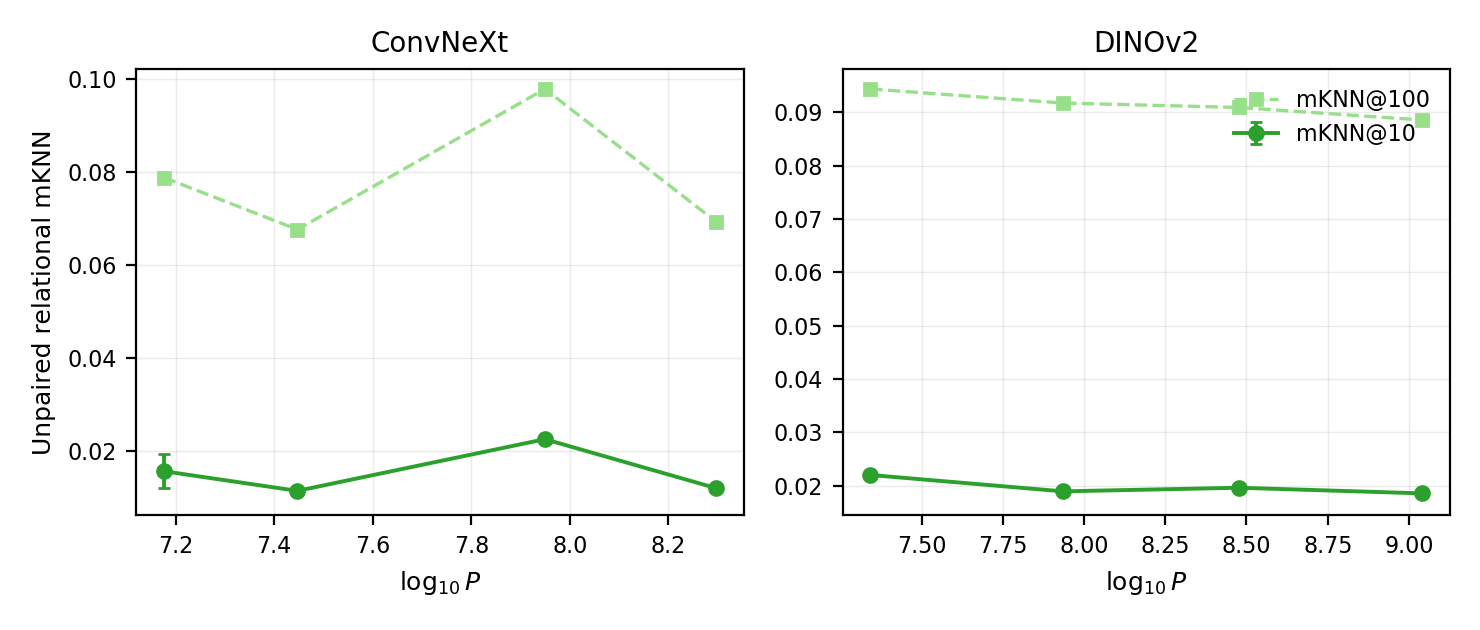
\includegraphics[width=0.92\linewidth]{figures/unpaired_legacy_mknn_vs_size.png}
\caption{Unpaired DualEncoder relational mKNN versus \(\log_{10}P\) (mean \(\pm\) seed sd).
Curves are non-monotonic across both available families.}
\label{fig:unpaired}
\end{figure}

\end{document}
